\documentclass[a4paper,reqno,oneside]{article} %amsbook ger en design mer lik den i boken, men är möjligen aningen för kompakt. article ger en mer luftig design med tydligare sektionsindelningar
%Options -- Point size:  10pt (default), 11pt, 12pt
%        -- Paper size:  letterpaper (default), a4paper, a5paper, b5paper
%                        legalpaper, executivepaper
%        -- Orientation  (portrait is the default)
%                        landscape
%        -- Print size:  oneside (default), twoside
%        -- Quality      final(default), draft
%        -- Title page   notitlepage, titlepage(default)
%        -- Columns      onecolumn(default), twocolumn
%        -- Equation numbering (equation numbers on the right is the default)
%                        leqno
%        -- Displayed equations (centered is the default)
%                        fleqn (equations start at the same distance from the right side)
%        -- Open bibliography style (closed is the default)
%                        openbib
% For instance the command
%           \documentclass[a4paper,12pt,leqno]{article}
% ensures that the paper size is a4, the fonts are typeset at the size 12p
% and the equation numbers are on the left side
%

% All package inclusions and defined commands go in this messy file:
\include{mathcommands.extratex}

\begin{document}

%%%%%%%%%%%%%%%%%%%
%%% Content from here on
%%%%%

\title{Excisiveness of graph clusterings?}
\author{Vilhelm Agdur}
\date{\today}
\maketitle

The goal in these notes is to take the results of \cite{carlsson_mémoli_2013}, which are in the setting of clustering generic finite metric spaces, and translate them into the setting of graphs, giving proofs that are free of the category-theoretical language.

\section{Definitions}

\begin{definition}
We will be concerned with two \emph{categories of finite simple graphs}, $\G^{inj}$ and $\G^{gen}$. In $\G^{inj}$, there is an arrow from $G$ to $H$ if $G$ is a subgraph of $H$, while in $\G^{gen}$ there is an arrow from $G$ to $H$ if we can identify some vertices of $G$ and end up with a subgraph of $H$.

Equivalently, the morphisms of $\G^{gen}$ are functions $f: V(G) \to V(H)$ such that for each edge $e = (a,b) \in E(G)$, either $f(a) = f(b)$ or $(f(a), f(b)) \in E(H)$, and in $\G^{inj}$ we require the morphisms to be injective, so only the latter possibility is allowed.\footnote{Note that we, in $\G^{gen}$, are allowed to send two vertices without an edge between them to the same vertex as well -- so in that category, the one-vertex graph is a final object. (In fact, it is a null object, since it is initial in both categories.)}
\end{definition}

\begin{definition}
A \emph{clustering scheme} is a function $\Clust$ that maps a finite simple graph to a partition of its vertices.

We say that a clustering scheme $\Clust$ is \emph{functorial with respect to $\G^{inj}$} if, whenever $G$ is a subgraph of $H$, $\Clust(G)$ is a refinement of $\Clust(H)|_G$.\footnote{Note that this is required to hold for \emph{every} way to realise the subgraph embedding of $G$ into $H$.} Equivalently, $\Clust$ is functorial (w.r.t $\G^{inj}$) if, whenever we add a new edge or a new vertex, $\Clust$ assigns the new vertex to some cluster, potentially a new one, and then potentially merges some clusters into larger clusters, but it never moves one vertex from one cluster to another or splits a cluster into smaller clusters.

We say that a clustering scheme $\Clust$ is \emph{functorial with respect to $\G^{gen}$} if the following holds: Whenever we have two graphs $G$ and $H$ and a $\G^{gen}$-morphism $f: G \to H$, $\Clust(G)$ is a refinement of $f^{-1}(\Clust(H))$. Here, we mean by $f^{-1}(\Clust(H))$ the partitioning of $G$ one gets by applying $f^{-1}$ to each part of $\Clust(H)$.

The ``generative'' picture of what $\G^{gen}$-functoriality means is the same as for $\G^{inj}$-functoriality, except that we need not only the requirement on adding edges or vertices, but also that whenever we identify two vertices, the same restrictions on how $\Clust(G)$ may change apply. In particular, this means that if we identify two vertices in two different clusters, the entire clusters must always merge.
\end{definition}

\begin{definition}
A clustering scheme $\Clust$ is \emph{excisive} if, whenever $H$ is a part of $\Clust(G)$, $\Clust(H|_H) = \{H\}$. That is, the clustering of a part of a clustering is just the part itself, so in a sense $\Clust$ is idempotent. 
\end{definition}

\begin{definition}
Let $\Omega$ be some fixed set of finite simple graphs. For any graph $G$ we can define a relation $\sim^{\Omega,inj}$ on its vertices by that $a \sim^{\Omega, inj} b$ if there exists a subgraph $H$ of $G$ containing both $a$ and $b$ which is isomorphic to some graph in $\Omega$. Equivalently, $a \sim^{\Omega,inj} b$ if there exists a graph $\omega \in \Omega$, vertices $\Tilde{a}, \Tilde{b} \in V(\omega)$, and a $\G^{inj}$-morphism $f: \omega \to G$ such that $f(\Tilde{a}) = a$ and $f(\Tilde{b}) = b$.

Likewise, we can define a relation $\sim^{\Omega,gen}$ on the vertices of $G$ in the exact same way, only replacing ``$\G^{inj}$-morphism $f$'' with ``$\G^{gen}$-morphism $f$''. Concretely, what this means is that we say that $a \sim^{\Omega,gen} b$ if there exists a subgraph $H$ of $G$ containing both $a$ and $b$ and a graph $\omega \in \Omega$ such that, after potentially identifying some vertices of $\omega$, $H$ and $\omega$ are isomorphic.

Now let $\sim^{\Omega,gen,*}$ be the least equivalence relation which contains $\sim^{\Omega,gen}$, that is, two vertices $a$ and $b$ are $\sim^{\Omega,gen,*}$-equivalent if there exist vertices $c_1, c_2,\ldots, c_n$ such that $a \sim^{\Omega,gen} c_1$, $c_{i-1} \sim^{\Omega,gen} c_i$ for $i = 2, 3, \ldots, n$, and $c_n \sim^{\Omega,gen} b$. Let $\Clust^{\Omega, gen}$ be the clustering scheme which assigns the clustering $V(G)/{\sim}^{\Omega,gen,*}$ to the graph $G$. We define $\Clust^{\Omega, inj}$ entirely analogously.

A clustering scheme $\Clust$ is \emph{$gen$-representable} if there exists an $\Omega$ such that $\Clust = \Clust^{\Omega,gen}$, and \emph{$inj$-representable} is defined entirely analogously.
\end{definition}

\section{The result}

The result, which holds in the finite metric space setting and we would like to show in this setting, is as follows:

\begin{theorem}\label{excisive_iff_representable}
A representable clustering scheme is excisive and functorial. A functorial and excisive clustering scheme is representable. These are the only implications that hold between these concepts.
\end{theorem}

This result holds equally well if we consider functoriality and representability over $gen$ as over $inj$, so we will omit specifying which we mean in our statements. We will divide the statement of this theorem into four lemmas, and prove them separately.

\begin{lemma}\label{representable_is_functorial}
A representable clustering scheme is functorial.
\begin{proof}
We start by considering the case of $inj$-functoriality and representability. Assume $\Clust = \Clust^\Omega$ for some set of finite simple graphs $\Omega$, and assume $G$ is some finite simple graph. What we need to show to show functoriality is that we, by adding an edge or a vertex to $G$, can only change the clustering of $G$ by merging clusters, and assigning the (potential) new vertex to an arbitrary, possibly new, cluster.

So let $G'$ be $G$ with an edge or a vertex added, and consider the definition of $\Clust^\Omega(G')$ -- it is precisely $V(G')/\sim^{G', \Omega, *}$. Now, $\sim^{G', \Omega, *}$ is the equivalence relation hull of the relation $\sim^{G', \Omega}$, so what we need to consider is how it may differ from $\sim^{G, \Omega}$. Since these relations are defined by the existence of a subgraph, and adding an edge or a vertex will not remove any subgraphs, two elements that are related under $\sim^{G, \Omega}$ will still be related under $\sim^{G', \Omega}$. Thus no two vertices will cease to be related under this relation when we add a vertex or edge, and thus the only change possible to the clustering is that two clusters merge, which is precisely what we needed to show to show functoriality.

For the case of $gen$-functoriality, the same argument nearly goes through, except we need to also allow the case where $G'$ is gotten from $G$ by identifying two of its vertices. This operation, however, will not make any vertices cease to be $\sim^{G, \Omega, gen}$-equivalent, since we in our definition precisely allowed for this case. To be concrete, let us assume that $a \sim^{G, \Omega, gen} b$ and show that $a \sim^{G', \Omega, gen} b$. Our assumption means that there exists some subgraph $H$ of $G$ and an $\omega \in \Omega$ such that, after potentially identifying some vertices of $\omega$, $H$ and $\omega$ are isomorphic. Now, if $H'$ is the same subgraph of $G'$, that is, $H$ with potentially two vertices identified, this must still be isomorphic to a version of $\omega$ with some vertices identified -- we may just need to make one additional identification of vertices in $\omega$ as well, and the same isomorphism still works. Thus, representability implies functoriality also in the case of $gen$. 
\end{proof}
\end{lemma}

\begin{lemma}\label{excisive_and_functorial_is_representable}
An excisive and functorial clustering scheme is representable.
\begin{proof}
Let $\Clust$ be an excisive clustering scheme, and let $\Omega$ be the set of all finite simple graphs $G$ such that $\Clust(G) = \{V(G)\}$, that is, the set of all graphs which are clustered as just a single part by $\Clust$. We claim that $\Clust = \Clust^{\Omega, inj} = \Clust^{\Omega, gen}$, so that $\Clust$ is representable in both senses.

So, let $G$ be an arbitrary finite simple graph, and let $a$ and $b$ be two vertices of $G$ which are clustered as belonging in the same part by $\Clust$. To see that they are also assigned to the same part by $\Clust^{\Omega, gen}$ and $\Clust^{\Omega,inj}$ it suffices to see that there exists a subgraph $H$ of $G$ containing $a$ and $b$ which is isomorphic to a graph in $\Omega$. This, however, is easy -- we can just take $H$ to be the entire part containing $a$ and $b$, and since $\Clust$ is excisive, it will cluster $H$ into just a single part, and thus $H$ is in $\Omega$.

Now, we instead take $a$ and $b$ to be two vertices of $G$ which are clustered as belonging in the same part by $\Clust^\Omega$, and show that they are also considered to be in the same part by $\Clust$. By definition, this must mean that there exists a sequence of vertices $c_1, \ldots, c_n$ such that $a \sim^\Omega c_1$, $c_{i-1} \sim^\Omega c_i$, and $c_n \sim^\Omega b$. So, if we can show that whenever two vertices are related by $\sim^\Omega$ they are clustered in the same part by $\Clust$, we will be done.

Let us first tackle the $inj$ case -- we have two vertices $a$ and $b$ such that $a \sim^{\Omega, inj} b$ and wish to show that they are in the same part according to $\Clust$. That $a \sim^{\Omega, inj} b$ means there exists some subgraph $H$ of $G$ containing both $a$ and $b$ which is isomorphic to some graph in $\Omega$. Since $H$ is in $\Omega$, we know that in particular $a$ and $b$ will be clustered in the same part in $\Clust(H)$, since $\Clust$ sends all of $H$ to one part. Then, if we add in edges and vertices one at a time to $H$, this will not change, since $\Clust$ is functorial -- so we can build all of $G$ around $H$ in this way, and in the end $a$ and $b$ must still be in the same part, which is what we wanted to show.

In the $gen$ case, the same argument essentially goes through, with only minor modification. Instead of getting a subgraph $H$ that is isomorphic to a graph in $\Omega$, we get a subgraph $H \ni a,b$ and a graph $\omega \in \Omega$, such that $H$ is isomorphic to $\omega$ potentially after identifying some vertices of $\omega$. Our ``generative'' argument works again, except we need to start in $\omega$ and identify a few vertices before we start building out to $G$. That the extra identifications do not split the part containing $a$ and $b$ is precisely the content of the extra strength of $gen$-functoriality compared to $inj$-functoriality.
\end{proof}
\end{lemma}

\begin{lemma}\label{lemma_representable_is_excisive}
A representable clustering scheme is excisive.
\begin{proof}
Let $\Clust$ be our clustering scheme and $\Omega$ be the set of graphs representing it. Consider some arbitrary graph $G$, and let $H$ be one of the parts of $\Clust(G)$ -- we wish to show that $\Clust(H) = \{V(H)\}$.

We will start with the $inj$ case. So, let $a$ and $b$ be two arbitrary vertices of $H$. That they are in $H$ means that they are in the same part in $G$, and so there must exist a sequence of vertices connecting $a$ to $b$ where each is related by ${\sim}^{G, \Omega, inj}$ to the next. So it is clear that if we can show that, for vertices in $H$, being ${\sim}^{G, \Omega, inj}$-related implies being ${\sim}^{H, \Omega, inj}$-related, the same chain will show that $a \sim^{H, \Omega, inj, *} b$, which will give us the result.

So, suppose that in fact $a \sim^{G, \Omega, inj} b$. This means there exists a subgraph $K$ of $G$, containing both $a$ and $b$, which is isomorphic to a graph in $\Omega$. If we could show that in fact $K \subseteq H$, we would be done. So, to see this, let $c$ be an arbitrary vertex of $K$ -- if we can show that in fact $c \sim^{G, \Omega, inj} a$ then $c$ must be in $H$ and we would be done. This, however, is obvious -- the subgraph $K$ itself demonstrates also this relation!

The same argument goes through essentially unchanged for the case of $gen$, as the reader easily verifies.
\end{proof}
\end{lemma}

\begin{lemma}
There are no other implications that hold between these three concepts.
\begin{proof}
To show this, we need to exhibit four examples: A clustering scheme that is functorial, representable, and excisive, a clustering scheme that is excisive but neither functorial nor representable, a clustering scheme that is functorial but neither representable nor excisive, and a clustering scheme that has none of the three properties. This will, together with our previous lemmas, completely fill out the $2 \times 2 \times 2$ table of possible combinations of properties with either examples or proofs of their impossibility.

\begin{table}[h]
    \begin{tabular}{l|ll}
        Functorial                         & \multirow{2}{*}{Excisive}       & \multirow{2}{*}{Not Excisive} \\ \cline{1-1}
        Not functorial                     &                                 &                               \\ \hline
        \multirow{2}{*}{Representable}     & \multicolumn{1}{l|}{Yes, Ex. \ref{ex_allthreeprops}} & No, by Lm. \ref{lemma_representable_is_excisive}                     \\
                                        & \multicolumn{1}{l|}{No, by Lm. \ref{representable_is_functorial}}   & No, by Lm. \ref{representable_is_functorial} (or by Lm. \ref{lemma_representable_is_excisive})            \\ \cline{2-3} 
        \multirow{2}{*}{Not Representable} & \multicolumn{1}{l|}{No, by Lm. \ref{excisive_and_functorial_is_representable}}   & Yes, Ex. \ref{ex_functnotexcnotrepr}                    \\
                                        & \multicolumn{1}{l|}{Yes, Ex. \ref{ex_excnotfunctnotrepr}} & Yes, Ex. \ref{ex_noprops}                   
    \end{tabular}
    \centering
    \label{table_twobytwobytwo}
    \caption{Table of all the possible combinations of properties, with examples or proofs of impossibility.}
\end{table}

\begin{example}\label{ex_allthreeprops}
For a scheme with all three properties, we can consider the connected components functor, which sends a graph to its set of connected components.
\end{example}

\begin{example}\label{ex_excnotfunctnotrepr}
For a scheme that is excisive but not functorial (and thus not representable), consider the scheme that partitions all graphs into a single part except the two-vertex one-edge graph, which it partitions into two parts.
\end{example}

\begin{example}\label{ex_functnotexcnotrepr}
For a scheme which is functorial but neither excisive nor representable, cluster all connected components on more than two vertices as well as all isolated vertices as their own parts. If there is exactly one component of two vertices, i.e. an isolated edge, cluster it as two parts, otherwise cluster all of them as single parts.
\end{example}

\begin{example}\label{ex_noprops}
Finally, a scheme which has none of the properties, cluster all graphs as a single part except for the two-vertex one-edge graph, which it clusters as two parts, and the disjoint union of two copies of that graph, which it clusters as two parts -- that is, each of the copies is its own part.
\end{example}

\end{proof}
\end{lemma}

Having shown this equivalence, let us now consider what the clustering schemes that actually have all three properties are. For the case of $gen$, the answer turns out to be very simple -- there is in fact only one non-trivial example.

\begin{theorem}\label{classifying_gen_representable}
Any $gen$-representable clustering scheme is one of:
\begin{enumerate}
    \item The scheme by which every vertex is its own part.
    \item The connected components functor.
    \item The scheme by which every graph is clustered as a single part.
\end{enumerate}
\begin{proof}
Consider some representable clustering scheme $C$, and let $\Omega$ be the set of graphs representing it.

If $\Omega = \emptyset$ or $\Omega$ contains only the one-vertex graph then we are clearly in case one.

If $\Omega$ contains some disconnected graph $\omega$, then for any graph $G$ and any $v, v' \in G$ we can just send one of the connected components of $\omega$ to $v$ and the rest to $v'$, exhibiting a relation between $v$ and $v'$. Since $v$ and $v'$ were arbitrary, this shows that $G$ is clustered into a single part.

So suppose $\Omega$ contains at least one graph on at least two vertices, and does not contain any disconnected graphs. Let $G$ be an arbitrary graph. To show that $C$ is the connected components functor, it suffices to show two things: That if $v$ and $v'$ are in different connected components of $G$ they are not related by $\sim^{G,\Omega,gen}$, while if there is an edge between them, they are.

That $v$ and $v'$ are not related if they are in different components is easy to see -- any graph $\omega$ exhibiting such a relation would have to be disconnected, since the distance between $v$ and $v'$ is infinite and the mapping sending $\omega$ into $G$ exhibiting the relation is distance non-increasing.

If there is an edge between $v$ and $v'$, pick some graph $\omega$ in $\Omega$ on at least two vertices, and send one of its vertices to $v$ and the rest to $v'$. That this does not increase any distances is easily seen, and so it is a $gen$-morphism, and this exhibits that $v$ and $v'$ are related, and so we are done.
\end{proof}
\end{theorem}

\begin{remark}
There are infinitely many distinct $inj$-representable clustering schemes. For example, let $\Clust_n$ be the clustering scheme represented by $\{K_n\}$. It is easy to see that whenever $n < m$, $\Clust_n$ will cluster $K_n$ as one part while $\Clust_m$ will cluster it with every vertex in its own part, since there is no injective function from $K_m$ into $K_n$. Thus $\Clust_n$ and $\Clust_m$ are distinct whenever $n\neq m$, and we have an infinite family of examples.
\end{remark}

It would be interesting to consider in more detail if we can classify what different $inj$-representable clustering schemes there are, because it is clearly true that we can have different sets of simple graphs represent the same clustering scheme.

\section{Other things to consider}

\begin{enumerate}
    \item Is there some way to describe these things in terms of graph minors, or find some intermediate between $gen$ and $inj$ described in those terms -- all the ``identifying vertices'' stuff pulls the mind in that direction. 
    \item \st{In the original paper, they have a Theorem 6.3 that classifies finitely representable clustering schemes -- I believe this result will not carry over, since it crucially involves defining an endofunctor that changes the metric on metric spaces, while we are rigidly stuck to the graph metric in our setting.} Actually it turns out to not just be true, but even true for all representable clustering schemes, not just \emph{finitely} representable clustering schemes -- which leads to the next question of:
    \item Are there \emph{any} representable but not finitely representable clustering schemes? There should be, but would be nice to have an example.
    \item \st{For similar reasons, their Theorem 6.4 would in our setting become the trivial statement that a clustering scheme that assigns to vertices to the same part iff there is an edge between them will just pick out the connected components.} Actually, this turned into Theorem \ref{classifying_gen_representable}.
    \item The things about scale invariance would also not translate well, I believe.
\end{enumerate}

\section{What about objective functions for clustering?}
We have considered assigning a single clustering to each graph, but it is also interesting to consider the problem of assigning a ``goodness'' score to each partition.

In fact, it might be interesting to consider assigning only a \emph{partial} ordering to the set of partitions of a graph, to reflect the fact that we for many graphs don't have any clear idea of what is \emph{the} best partition, only some ideas that some are better than others. (Think paramagnetic phase and so on -- lots of fancy words could be put here. In particular the example in the first figure of \cite{moore_2017} is what I'm thinking of.)

So, let us begin defining our categories that are involved. (We will use slightly different notation than in the previous notation -- because I don't want to go back to change the notation there before I know if this section results in anything interesting.)

\subsection{Categories of graphs}

\begin{definition}
A simple graph $G$ is a pair of a finite set $V(G)$ and a symmetric reflective relation $E(G)$ on the set $V(G)$. We denote ``elements $v$ and $w$ of $V(G)$ are related via $E(G)$'' (i.e., there is an edge between $v$ and $w$) by $v \sim w \in E(G)$.\footnote{Technically we should perhaps write $(v,w) \in E(G)$?} 
\end{definition}

\begin{definition}
Let $\mathrm{SimpGph}$ be the category whose objects are simple graphs, and morphisms $G \to G'$ are maps $f: V(G) \to V(G')$ such that whenever there is an edge $v \sim w \in E(G)$, we also have $f(v) \sim f(w) \in E(G')$.

Let $\mathrm{MonoSimpGph}$ be the wide subcategory of $\mathrm{SimpGph}$ where we only keep the injective morphisms, and $\mathrm{RegMonoSimpGph}$ be the wide subcategory of $\mathrm{MonoSimpGph}$ where we only keep the morphisms which are isomorphisms onto their image.
\end{definition}

\begin{definition}
Take two graphs $G$ and $G'$, and a morphism $f \in \mathrm{Hom}_{\mathrm{SimpGph}}(G, G')$, and consider the set of fibers $\Delta = \left\{f^{-1}(v')\given v' \in V(G')\right\}$. If each $\delta \in \Delta$ is an independent set in $G$, and for every pair $\delta, \Tilde{\delta}$ of fibers, $E(\delta,\Tilde{\delta}) = \left\{v \sim w \in E(G) \given v \in \delta, w \in \Tilde{\delta}\right\}$ has cardinality zero or one, we say that $f$ is \emph{edge-injective}, or that it is \emph{a monomorphism on the edges}.
\end{definition}

\begin{remark}
Notice that, in the notation of the previous definition, there exists a natural multigraph structure on $\Delta$, where we put $\abs{E(\delta,\delta')}$ edges between $\delta$ and $\delta'$, and $\abs{\left\{v \sim w \in E(G) \given v, w \in \delta\right\}}$ loops at $\delta$. If we simplify this multigraph to a graph, we get precisely the image of $f$. Being injective on the edges is then the statement that this multigraph is in fact already a simple graph.

If we had defined a simple graph as a set of vertices along with a set of edges (satisfying some conditions to make sure the graph is simple), being injective on the edges would mean precisely that the induced function from $E(G)$ to $E(G')$ was injective, justifying the choice of terminology.
\end{remark}

\begin{lemma}\label{lemma_mu_morphisms_compose}
Suppose $f \in \mathrm{Hom}_{\mathrm{SimpGph}}(G, G')$ and $g \in \mathrm{Hom}_{\mathrm{SimpGph}}(G', G'')$ are both injective on the edges. Then $f \circ g \in \mathrm{Hom}_{\mathrm{SimpGph}}(G, G'')$ is also injective on the edges.\footnote{The statement may sound nearly trivial with this choice of notation, since obviously compositions of injective maps are injective, but since we haven't actually defined the concept as just being an injective map, we do need to verify that this holds.}
\begin{proof}
Let $\Delta_f \in \mathcal{P}(\mathcal{P}(V(G)))$ be the set of fibers of $f$, $\Delta_g \in \mathcal{P}(\mathcal{P}(V(G')))$ be the set of fibers of $g$, and $\Delta_{fg} \in \mathcal{P}(\mathcal{P}(V(G)))$ the set of fibers of $f\circ g$. We need to show two things -- that each element of $\Delta_{fg}$ is an indepedent set, and that for each pair of elements of $\Delta_{fg}$, there is only one or zero edges between them.

So, pick a $\delta \in \Delta_{fg}$, and suppose for contradiction that this $\delta$ is not an independent set, so that there exist $v_1, v_2 \in \delta \subseteq V(G)$ such that $v_1 \sim v_2 \in E(G)$. Now, if $f(v_1) = f(v_2)$, this would violate the assumption that $f$ is injective on the edges, since this would imply that the fiber of $f$ in which $v_1$ and $v_2$ are is not an independent set. However, if instead $f(v_1) \neq f(v_2)$, we would have $f(v_1) \sim f(v_2) \in E(G')$, since $f$ is a graph morphism -- but since by assumption $v_1$ and $v_2$ are in the same fiber of $f\circ g$, we must have $g(f(v_1)) = g(f(v_2))$, and so $f(v_1)$ and $f(v_2)$ are in the same fiber of $g$. This however means we have found two vertices in the same fiber of $g$ which have an edge between them, violating the assumption that all fibers of $g$ are independent sets. Thus, we have our contradiction.

Now, pick two fibers $\delta, \gamma \in \Delta_{fg}$, and assume for contradiction that there exist at least two edges between them. That is, we have distinct vertices $v_\delta, w_\delta \in \delta$ and $v_\gamma, w_\gamma \in \gamma$ such that $v_\delta \sim v_\gamma \in E(G)$ and $w_\delta \sim w_\gamma \in E(G)$.

Now, there are two different possibilities, either $f(v_
\delta) = f(w_\delta)$ and $f(v_\gamma) = f(w_\gamma)$, or at least one pair remains unidentified by $f$

\begin{figure}[h]
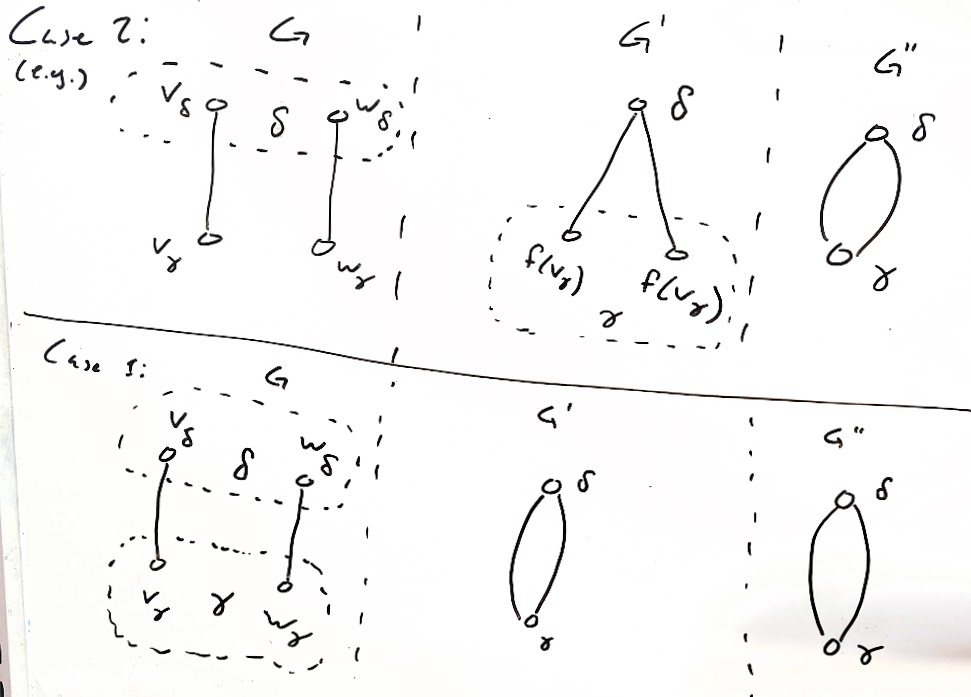
\includegraphics[width=8cm]{graphics/figure_mu_morphisms_compose.jpg}
\centering
\label{fig_mu_morphisms_compose}
\caption{Pictorial representation of what is going on in the second half of the proof of Lemma \ref{lemma_mu_morphisms_compose}}
\end{figure}

In the first case, this means that in fact $v_\delta$ and $w_\delta$ are in the same fiber of $f$, and likewise for $v_\gamma$ and $w_\gamma$. But this means that these two fibers of $f$ have more than one edge between them, violating the assumption that $f$ is injective on the edges.

In the second case, assume wlog that $v_\delta$ and $w_\delta$ did not get identified. Since $f$ is a graph morphism, we must have $f(v_\delta) \sim f(v_\gamma) \in E(G')$ and $f(w_\delta) \sim f(w_\gamma) \in E(G')$, and these must be distinct edges. But by assumption, $g(f(v_\delta)) = g(f(w_\delta))$ and likewise for the $\gamma$-indexed ones, since we assumed they were in the same fiber of $f\circ g$. So this means that we have found two fibers of $g$ with more than one edge between them, violating our assumption that $g$ is injective on the edges.

This finishes the proof.
\end{proof}
\end{lemma}

Having established this lemma, we can make the following definition:\footnote{Without it, we wouldn't know that the morphisms composed in the right way.}
\begin{definition}
Let $\mathrm{EdgeMonoSimpGph}$ be the wide subcategory of $\mathrm{SimpGph}$ whose morphisms all have property $\mu$.
\end{definition}

\begin{remark}
It is easy to see that we have
$$\mathrm{RegMonoSimpGph} \subsetneq \mathrm{MonoSimpGph} \subsetneq \mathrm{EdgeMonoSimpGph} \subsetneq \mathrm{SimpGph}$$
\end{remark}

\subsection{Categories of partitions}

Throughout this section, $P < P'$ for set partitions $P$ and $P'$ will always mean that $P$ is a refinement of $P'$. 

\begin{definition}
The category $\mathrm{PartSet}$ of partitioned sets has as objects tuples $(V,P)$ where $V$ is a finite set and $P$ is a set partition of $P$. A morphism $f: (V, P) \to (V', P')$ is a set function $f: V \to V'$ such that $P < f^*(P') = \left\{f^{-1}(A) : A \in P'\right\}$.
\end{definition}

This definition was latent in our discussion of clustering schemes that assign just a single partition to each graph -- a clustering scheme being functorial meant precisely that it was a functor from $\mathrm{SimpGph}$ to $\mathrm{PartSet}$, or from $\mathrm{MonoSimpGph}$, if we meant in the sense of $inj$.

So, since we want to study clustering schemes that rank the different options for clustering, we should introduce a category for these as well. For any set $V$, let $P(V)$ denote the set of set partitions of $V$, and let $OP(V)$ denote the set of partial orders on $P(V)$. To make our notation more readable, if we have a function $\hat{f}: OP(V) \to OP(V')$, we will write $\prec_{\hat{f}}$ instead of $\hat{f}(\prec)$ for the image of $\prec \in OP(V)$ under $\hat{f}$, since $P' \prec_{\hat{f}} Q'$ is vastly more readable than $P' \hat{f}(\prec) Q'$.

If we have a function $f: V \to V'$, this induces a function $f^*: P(V') \to P(V)$ by setting $f^*(P') = \left\{f^{-1}(A_i) \given A_i \in P'\right\}$. It also induces a function $\hat{f}: OP(V) \to OP(V')$, which we get by that $P' \prec_{\hat{f}} Q'$ if and only if $f^*(P') \prec f^*(Q')$.

If we have two partial orders $\prec$ and $\preccurlyeq$ in $OP(V)$, we say that $\preccurlyeq$ is a \emph{tightening} of $\prec$ if for all $P$ and $Q$ in $P(V)$,
$$(P < Q) \rightarrow (P \prec Q \rightarrow P \preccurlyeq Q),$$
that is, whenever $P$ is finer than $Q$ and also worse than $Q$ according to $\prec$, it will also be worse than $Q$ according to $\preccurlyeq$.

With all these definitions and notations in hand, we can define the category we are interested in:

\begin{definition}
The category $\mathrm{OrdPartSet}$ has as objects tuples $(V, \prec)$ of a set $V$ and a partial order $\prec$ on the set of set partitions of $V$. A morphism from $(V,\prec)$ to $(V', \prec')$ is a set function $f: V \to V'$ such that $\prec'$ is a tightening of $\hat{f}(\prec)$.\footnote{\hl{Check that this is the right relation, that it isn't the opposite we want -- too late at night to check again right now when writing it.}}
\end{definition}

Expanding what the definition actually means, if $f$ is a morphism from $(V,\prec)$ to $(V',\prec')$, this means that for any two partititions $P'$ and $Q'$ of $V'$ where $P' < Q'$, if $f^*(P') \prec f^*(Q')$ then $P' \prec' Q'$.

Just like we defined some wide subcategories of $\mathrm{SimpGph}$, we will want to define some subcategories of $\mathrm{OrdPartSet}$, but now it makes more sense to create some \emph{full} subcategories.

\begin{definition}
Let $\mathrm{TopOrdPartSet}$ be the full subcategory of $\mathrm{OrdPartSet}$ whose objects all have \emph{topped} orders, that is, orders with a maximal element. Let $\mathrm{LatOrdPartSet}$ be the full subcategory of $\mathrm{TopOrdPartSet}$ whose objects all have orders which are lattices, and finally let $\mathrm{TotOrdPartSet}$ be the full subcategory of $\mathrm{LatOrdPartSet}$ whose objects all have \emph{total} orders.
\end{definition}

\begin{lemma}
$\mathrm{OrdPartSet}$, and thus also all the subcategories we defined, is a category.
\begin{proof}
Almost every condition is trivially fulfilled, and the notion of composition of morphisms is obvious -- but we do need to verify that the composition of two morphisms is still a morphism.

So, suppose we have
$$(V, \prec) \xrightarrow{f} (V', \prec') \xrightarrow{g} (V'', \prec'')$$
where $f$ and $g$ are both morphisms in $\mathrm{OrdPartSet}$. We wish to show that $f\circ g$ is a morphism from $(V, \prec)$ to $(V'',\prec'')$.

That is, we want to consider two partitions $P''$ and $Q''$ of $V''$, such that $P'' < Q''$ and $f^*(g^*(P'')) \prec f^*(g^*(Q''))$, and show that we then have that $P'' \prec'' Q''$.

Since $P'' < Q''$ we must have that $g^*(P'') < g^*(Q'')$. We have by assumption that $f^*(g^*(P'')) \prec f^*(g^*(Q''))$, and thus, since $f$ is an $\mathrm{OrdPartSet}$-morphism, we get that $g^*(P'') \prec' g^*(Q'')$. But now we can use this fact together with that $P'' < Q''$ and that $g$ is an $\mathrm{OrdPartSet}$-morphism to see that $P'' \prec'' Q''$, which is exactly what we wanted to see.
\end{proof}
\end{lemma}

For $\mathrm{TopOrdPartSet}$ there exists an obvious map $Top$ from its objects to the objects of $\mathrm{PartSet}$, which sends the pair $(V,\prec)$ to the pair $(V,\max \prec)$, that is, $V$ together with the partition that is maximal according to $\prec$.

\begin{remark}\label{remark_top_not_functor}
$Top$ does \emph{not} define a functor from $\mathrm{TotOrdPartSet}$ to $\mathrm{PartSet}$, and thus also does not define a functor from $\mathrm{LatOrdPartSet}$ or $\mathrm{TopOrdPartSet}$ to $\mathrm{PartSet}$.
\begin{proof}
Choose an arbitrary $n$, and let $P_i = \{\{i\},[n]\setminus \{i\}\}$, for $i = 1, \ldots, n$. Let $\ll$ be some arbitrary total order on $P([n])$. We define an ordering $\prec$ on $OP([n])$ by that
\begin{itemize}
    \item For all $1\leq i < j \leq n$, $P_i \prec P_j$.
    \item For any $P$ that is not of the form $P_i$ for any $i$, $P \prec P_i$.
    \item If neither $P$ nor $Q$ is of the form $P_i$, $P \prec Q$ iff $P \ll Q$.
\end{itemize}
and an ordering $\prec'$ by the same statements, except we flip the ordering of the $P_i$, so that $P_i \succ' P_j$ whenever $i < j$.

We claim that the identity map on $[n]$ mapping $([n],\prec)$ to $([n],\prec')$ is a morphism in $\mathrm{TotOrdPartSet}$, but that the identity mapping from $([n], P_n)$ to $([n],P_1)$ is not a morphism in $\mathrm{PartSet}$. This will suffice to show that $Top$ is not a functor.

That both $\prec$ and $\prec'$ are total orders is easy to see, so we need only verify that $f = \mathrm{Id}$ is a morphism. Since our $f$ is just the identity function on a set, our definition simplifies to the following: For any two partitions $P$ and $Q$ of $[n]$, such that $P$ is a refinement of $Q$ and $P \prec Q$, it has to also hold that $P \prec' Q$.

There are three cases: Neither $P$ nor $Q$ is of the form $P_i$, one is but the other is not, or both are of that form.

If neither $P$ nor $Q$ is of the form $P_i$, then $\prec$ and $\prec'$ will by construction agree on how to order them, and our condition will be fulfilled.

If $P \prec Q$ and $Q = P_i$ for some $i$, but $P$ is not of that form, then again $\prec$ and $\prec'$ will agree that $Q$ is greater than $P$, and so our condition is fulfilled.

If $P = P_i$ and $Q = P_j$, then neither is a refinement of the other, and so our condition imposes no restrictions, and is trivially fulfilled.

So, we have seen that we have a morphism in $\mathrm{TotOrdPartSet}$. It remains to see that, when we map this forward into $\mathrm{PartSet}$, we do not get a morphism. By our definition of a morphism in $\mathrm{PartSet}$, we would have to have that $P_n < P_1$, which is clearly not the case, and so we are done. 
\end{proof}
\end{remark}

\subsection{Representability}
We found the notion of a representable clustering scheme to be interesting in the previous section, so let us try to define an analogous notion in the current setting.

\begin{definition}
Given any not necessarily finite set of finite simple graphs $R$, we can define an endofunctor $F_R$ on $\mathrm{SimpGph}$ as follows:

Given a graph $G = (V,E)$, $F_R(G) = (V, H)$, where $(v,w) \in H$ if there exists an $\omega \in R$ and a morphism $f: \omega \to G$ such that $\im \omega \ni v, w$. For any morphism $f: (V,E) \to (V',E')$, $F_R(f)$ is just the same set function $f: V \to V'$ again.

The same definition of course makes sense for any of our subcategories of $\mathrm{SimpGph}$, where we just need to require the morphism $f$ to also lie in that subcategory.
\end{definition}

\begin{lemma}\label{lemma_repr_endofunctor_is_functor}
The endofunctor $F_R$ is actually a functor for every set of simple graphs $R$, for $\mathrm{SimpGph}$ and for all of our subcategories.

\begin{proof}
That $F_R$ is well defined, always sends graphs to graphs, and respects composition at the set function level is obvious for each of our categories. What we need to show is that, for each of our categories, if $f: (V,E) \to (V',E')$ is a morphism, then $F_R(f)$ actually is a morphism from $F_R((V,E)) = (V,H)$ to $F_R((V',E')) = (V',H')$.

So, to see this, take two arbitrary vertices $v, w \in V$ such that $(v,w) \in H$ -- we want to show that this implies that $(f(v),f(w)) \in H'$. Now, that $(v,w) \in H$ implies that there exists an $\omega \in R$ and a morphism $g: \omega \to G$ such that $\im \omega \ni v, w$. Then, however, we easily see that by composing $f$ and $g$ we get a morphism $g \circ f: \omega \to G'$ whose image contains $f(v)$ and $f(w)$, showing that $(f(v),f(w)) \in H'$, as desired. Note that this argument works in any of our categories, as long as we shift the meaning of the word ``morphism'' to be in the appropriate category.
\end{proof}
\end{lemma}

\begin{remark}
Note that Lemma \ref{lemma_repr_endofunctor_is_functor}, together with the observation that the connected components functor is indeed a functor from $\mathrm{SimpGph}$ into $\mathrm{PartSet}$, provides a much cleaner proof of Lemma \ref{representable_is_functorial}, at the expense of introducing some more terminology.
\end{remark}

The preceding remark should motivate us to try to find a definition of a representable partial order clustering scheme by finding an analogue of the connected components functor going from $\mathrm{SimpGph}$ into $\mathrm{OrdPartSet}$ instead of into $\mathrm{PartSet}$. First, however, let us try to understand these $F_R$ somewhat better.

\begin{lemma}\label{lemma_hulls_of_representable_endofunctors}
For any set of simple graphs $R$ and any simple graph $G = (V_G,E_G)$, it holds that $F_R = F_{R \cup \{G\}}$ iff $F_R(G) = (V_G, V_G^2)$, that is, adding $G$ into $R$ leaves the endofunctor $F_R$ unchanged if and only if $F_R$ already sent $G$ to a clique graph.

\begin{proof}
Suppose $F_R(G) = (V,V^2)$, and let $H = (V_H, E_H)$ be an arbitrary graph. We wish to show that $F_{R\cup\{G\}}(H) = F_R(H)$. By definition of $F_R$ it is easy to see that $F_{R\cup\{G\}}(H)$ must be a subgraph of $F_R(H)$, since there appears an edge whenever we can map a ``test graph'' $\omega \in R$ into $H$ in the right way, and so adding more test graphs can't possibly remove an edge. So it suffices to show that whenever $(v,w)$ is an edge of $F_{R\cup\{G\}}(H)$ it was already an edge of $F_R(H)$.

Now, if $(v,w)$ is an edge of $F_{R\cup\{G\}}(H)$, that means by definition that there exists an $\omega \in R \cup \{G\}$ and a morphism $f: \omega \to H$ such that $v, w \in \im f$. If $\omega$ is already in $R$, then we are done, so we can assume $\omega = G$. Pick $v', w' \in V_G$ such that $f(v') = v$ and $f(w') = w$. Since we assumed $F_R$ sends $G$ to a clique, $(v', w')$ must be an edge of $F_R(G)$, and so there exists an $\omega' \in R$ and a $g: \omega' \to G$ such that $v', w' \in \im g$ -- but now the composition $g \circ f: \omega' \to H$ is a morphism from an element of $R$ into $H$ which hits $v$ and $w$ (since $f(v') = v$ and $f(w') = w$), which shows that $(v,w)$ was in fact already an edge of $F_R(H)$.

For the other direction, we show the contrapositive, that if $F_R$ does not send $G$ to a clique then $F_{R\cup\{G\}} \neq F_R$. To start with, note that for any $\omega \in R$, $F_R$ must send $\omega$ to a clique -- since the identity map on $\omega$ trivially has every vertex in its image, there must be an edge between every pair of vertices. So we must have that $F_{R\cup\{G\}}(G) = (V_G, V_G^2)$, and by assumption $F_R$ did not send $G$ to a clique, and so $F_{R\cup\{G\}}(G) \neq F_R(G)$, showing that they are not equal.
\end{proof}
\end{lemma}

\begin{remark}
It is not true in $\mathrm{MonoSimpGph}$ that every $F_R$ is equal to some $F_{R'}$ for a finite set $R'$, that is, not all representable endofunctors are \emph{finitely} representable. \hl{I think there's a simpler and sharper example that gets also non-injective morphisms, but too sleepy to write it out right now. Essentially the number of edges argument again, and just use $R$ as paths.}
\begin{proof}
For each $n \geq 3$, let $\Delta_n$ be the graph whose vertex set is $[n]$, and which has edges between $i$ and $i+1$ for $i = 1,\ldots, n-1$, and also an edge from $1$ to $3$. That is, $\Delta_n$ is a triangle with a tail. Let $R$ be the set of all $\Delta_n$. We claim that $F_R$ is not finitely representable.

First, let $\Bar{R}$ be the set of graphs which $F_R$ sends to a clique -- a bit of thought will reveal that $\Bar{R}$ is exactly the set of connected graphs which contain a triangle. By Lemma \ref{lemma_hulls_of_representable_endofunctors} $F_R = F_{\Bar{R}}$, so we may as well show that $F_{\Bar{R}}$ is not finitely representable.

So, suppose for contradiction that $F_{R'} = F_{\Bar{R}}$ for some finite set $R'$. It is not too hard to see that we must have $R' \subset \Bar{R}$, since if there were an $\omega \in R' \setminus \Bar{R}$, then it would be sent to a clique by $F_{R'}$ but not by $F_{\Bar{R}}$, since $\omega \not\in \Bar{R}$ and $\Bar{R}$ contains every graph sent to a clique by $F_{\Bar{R}}$.

Since $R'$ is finite, we can let $N_e = \max_{\omega \in R'} \abs{E_\omega}$ be the highest number of edges any graph in $R'$ has. We claim that $\Delta_{N_e+3}$ will not be sent to a clique by $F_{R'}$, because there will not be an edge between $N_e+2$ and $N_e+3$. To see this, consider what could cause such an edge to exist -- a morphism sending some $\omega \in R'$ into $\Delta_{N_e+3}$ that hits the final vertices on its tail. But the $\omega$ would contain a triangle, since $\omega \in R' \subset \Bar{R}$ and everything in $\Bar{R}$ contains a triangle, and since we assume our morphisms are injective this triangle has to be sent to the triangle in $\Delta_{N_e+3}$. But this triangle is simply too far away -- there aren't enough edges in $\omega$ to both hit the end of the tail and the triangle. So $\Delta_{N_e+3}$ can't be sent to a clique, establishing that $F_{R'} \neq F_R$, as desired.
\end{proof}
\end{remark}

\hl{Lemma} \ref{classifying_gen_representable} \hl{essentially shows that for $\mathrm{SimpGph}$, there are actually only three distinct representable functors \emph{when we postcompose with the connected components functor}, and those three are all finitely representable. I think this can be turned into the statement that a representable endofunctor on $\mathrm{SimpGph}$ always sends a graph to a supergraph of itself if $R$ is nonempty.}

\begin{definition}
We use $\Pi$ for the connected components functor from $\mathrm{SimpGph}$ to $\mathrm{PartSet}$, which sends a graph to the partitioning of its vertices into its connected components. Note that a ``representable clustering scheme'' in the first half is then just a clustering scheme which can be written as $F_R \circ \Pi$ for some set of graphs $R$.

We use $\Delta$ for the ``cliqueifying'' functor from $\mathrm{PartSet}$ to $\mathrm{SimpGph}$ which sends $(V,P)$ to $(V,E)$, where $(v,w) \in E$ iff $v$ and $w$ are in the same part in $P$. 
\end{definition}

\hl{I think $\Pi$ and $\Delta$ should be adjoint, whatever that really means, and this in turn somehow connects to the observation that a graph is completely determined by the morphisms from $K_2$ into it? Should explore this further.}

\subsection{Excisiveness}
We want to extend not just our notion of representability but also the notion of excisiveness to the setting of functors into $\mathrm{OrdPartSet}$.

\begin{definition}
A functor $\Clust$ from $\mathrm{SimpGph}$ into $\mathrm{OrdPartSet}$ is \emph{order-excisive} if it holds for every graph $G = (V,E)$ that, for every partition $P = \{A_1, A_2,\ldots, A_n\}\in P(V)$ and every pair of partitions $B = \{B_1,\ldots,B_{n_B}\}$ and $C = \{C_1, \ldots, C_{n_C}\}$ in $P(A_1)$, whenever $B \prec_{\Clust(G|_{A_1})} C$,\footnote{Where we by $G|_{A_1}$ mean the induced subgraph of $A_1$ in $G$.} we also have $\{B_1, \ldots, B_{n_B}, A_2, \ldots, A_n\} \prec_{\Clust(G)} \{C_1, \ldots, C_{n_C}, A_2,\ldots A_n\}$. The same definition of course also makes sense replacing either category with one of its subcategories.
\end{definition}

To motivate why we call this a version of excisiveness, we have the following lemma:
\begin{lemma}
If $\Clust$ is an order-excisive functor from $\mathrm{SimpGph}$ to $\mathrm{TopOrdPartSet}$, the composition of $\Clust$ with $Top$, the map that sends a pair of a set $V$ and a topped order on $OP(V)$ to the pair of the set and the maximal element of the order, will be an excisive (but not necessarily functorial, cf. Remark \ref{remark_top_not_functor}) clustering scheme.
\begin{proof}
Let $G$ be some arbitrary graph, and let $P = \{A_1, \ldots, A_n\}$ be the maximal clustering of $G$ according to $\prec_{\Clust(G)}$. We need to show that $\{A_1\}$ will be the maximal clustering of $G|_{A_1}$. So suppose for contradiction that there is some better partitioning $B = \{B_1, \ldots, B_m\}$ of $A_1$, that is, that there is a $B$ such that $\{A_1\} \prec_{\Clust(G|_{A_1})} B$. Then, since $\Clust$ is order-excisive by assumption, this must mean that $A = \{A_1, A_2, \ldots, A_n\} \prec_{\Clust(G)} \{B_1, \ldots, B_m, A_2,\ldots A_n\}$ -- but we assumed that $A$ was the maximal element of $\prec_{\Clust(G)}$, and so we have our desired contradiction.
\end{proof}
\end{lemma}

\printbibliography

\end{document}